\documentclass[a4paper,10pt]{report}
\usepackage[utf8]{inputenc}
\usepackage{graphicx}


% Title Page
\title{\textbf{OPTICAL COMMUNICATION COMPONENTS \\ Lab 1}}
\author{Nicola Simoni, Tadewos Somano}
\date{University of Brescia, Faculty of Engineering\\A.Y. 2013-2014}


\begin{document}
\maketitle


\section*{Question 1}
The difference between the two scope traces resides in the power. In fact both signals have the same waveform but
the power of the positive pulse of the first signal is about 5 $mW$, while the one of the second is about 5 $\mu W$, that is three order
of magnitude smaller.

\section*{Question 2}
The electrical received signal is severely distorted because of the photo-detector. In fact, even if the optical signal is undistorted, the
photo-detector introduces thermal noise. Moreover, smaller the power received, more severe is the effect of the noise.

\section*{Question 3}
In Figure \ref{plot} is shown the curve that represents the bit error rate (BER) as a function of the distance.
The red dots on the plot represent the values computed at given distances, while the blue line is the linear interpolation of the points.
The BER axis is in logarithmic (base 10) scale, while the distance axis is in linear scale.
Assuming that the maximum acceptable BER is $10^{-9}$ (which logarithm is -9), the corresponding distance
is nearly 144 Km. So, to have acceptable BER, the maximum length of the link has to be lower or equal than this value.
%This means that we have to use distances lower than this value if we want to have an acceptable bit error rate.
In Figure \ref{plotzoom} is shown the limit point, indicated by the black arrow.

\begin{figure}[!h]
  \centering
  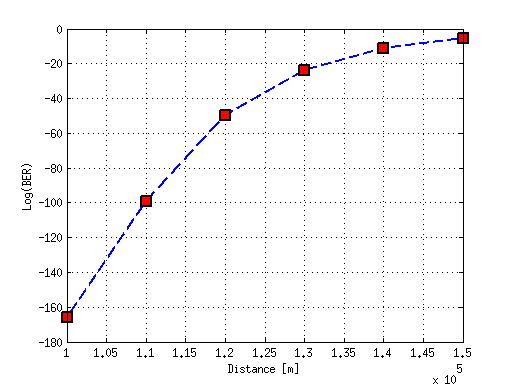
\includegraphics[width=12cm]{plot.png}\\
  \caption{BER versus distance.}
  \label{plot}
\end{figure}


\begin{figure}[!ht]
  \centering
  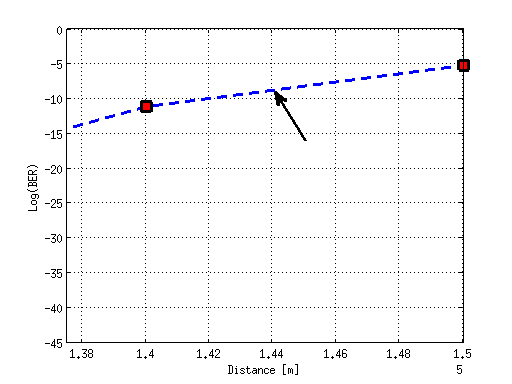
\includegraphics[width=12cm]{plotzoom.png}\\
  \caption{Limit point.}
  \label{plotzoom}
\end{figure}


\section*{Question 4}
To overcome loss limit is not possible to increase the power arbitrarily. In fact we have to take into account dispersion, that is a linear
effect that causes the spreading of the signals transmitted and doesn't depend on the power.

\end{document}